The geometry will be representative of a tokamak cross-section, possibly
omitting
the region containing the central hot plasma, so that topologically it
will be at most as complex as an annulus (one-hole). \Fig{xsect}
provides an example. 
The Last Closed Flux Surface~(LCFS) may be parameterised by arc-length
in the cross-sectional plane of projection.

\begin{figure}
\centerline{
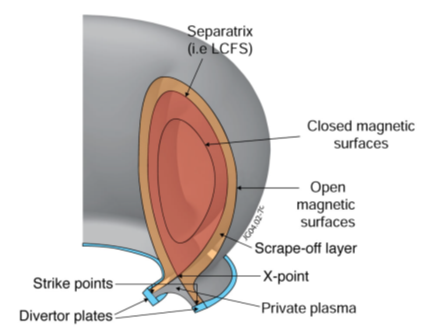
\includegraphics[width=8.0cm]{../png/xsect.png}
}
\caption{Sketch of the test configuration, showing tokamak cross-section
and the boundary of the Last Closed Flux Surface (LCFS).
\label{fig:xsect}}
\end{figure}

The elliptic equations to be considered now follow.

\subsection{Simplified Grad-Shafranov equation} \label{sec:GSimp}
This elliptic equation is a simplified version
of the Grad-Shafranov equation, see \cite{Ap18Equi}
\begin{equation}\label{eq:gs}
R^2 \nabla \cdot \frac{1}{R^2} \nabla \psi = -2 \mu_0 R j_{\phi}
\end{equation}
where $\psi$ is the poloidal magnetic flux and $(R,Z)$ are cylindrical coordinates
in planes normal to the toroidal direction~$\phi$, with the toroidal current
\begin{equation}\label{eq:jphi}
j_\phi= R \frac{dp(\psi)}{d\psi}+ \frac{I}{\mu_0 R} \frac{dI(\psi)}{d\psi} + j_{ext}(R,Z)
\end{equation}
The functions~$p$ and~$I$ give the variation as functions of~$\psi$
of the pressure and toroidal field respectively, and $j_{ext}(R,Z)$
may be produced in several ways, of which the commonest is by
poloidal field circuits, ie.\ localised current sources in cross-section.
Note that the operator in \Eq{gs} simplifies to
\begin{equation}\label{eq:gsimp}
\frac{\partial^2}{\partial R^2} - \frac{1}{R}  \frac{\partial}{\partial R} + \frac{\partial^2}{\partial Z^2}
\end{equation}
which implies that mathematically, $\psi$ satisfies a steady-state 2-D advection-diffusion
equation corresponding to unit diffusivity in the flow $u_R=1/R$.

To provide the simple test case, take $j_\phi=j_{ext}$ only with localised current sources.
The boundary conditions are $\psi=0$ on the LCFS
and $\psi \propto 1/\sqrt(R^2+Z^2)$ as $R,\;Z \rightarrow \infty$.

Note that the Grad-Shafranov equation has been solved using spectral elements by
others, eg.\ Sovinec~\cite{Ho14Solv}.
%so that $\psi$ decreases outwards from the LCFS

\subsection{Simplified non-Boussinesq vorticity equation} \label{sec:boussimp}
A simplified version of the non-Boussinesq vorticity equation to be solved for
the scalar field $\Phi(R,Z)$ in cylindrical polar coordinates~$(R,Z)$ is
\begin{equation}\label{eq:ellsimp}
\nabla_\perp \cdot \left( \frac{1}{B^2}  \nabla_\perp \Phi \right) = n
\end{equation}
where $B=|{\bf B}|$ is the amplitude of the imposed magnetic field,
density~$n$ acts as a source term, and the elliptic is to be solved
for~$\Phi$, subject to boundary conditions $\Phi=0$. The operator $\nabla_\perp$,
ignoring the components of magnetic field directed within the $(R,Z)$~plane,
reduces to the usual gradient~$\nabla$ in cylindrical polars of axisymmetric
fields, hence mathematically \Eq{ellsimp}
is equivalent to~\Eq{gs}.

$n$ will be set so that $n=n_0(s_i)$ on the boundaries,
where arc-length~$s_i$
parameterises the inner boundary if $i=1$ and the outer if $i=2$.
$n$ and $|B|$ will be specified functions of $(R,Z)$ that capture features
of the number density~$n$ distribution and magnetic field intensity distribution
expected in a tokamak,
Ideally $|B|$ would represent a solution of the Grad-Shafranov equation from \Sec{GSimp}.
